\chapter{Experiments and Results}
\label{chapter:results}

Now that we have discussed several feature extraction methods and alternate
language model architectures, it is time to put to test these proposals and
evaluate how well they perform on the captioning task.
%%
In this chapter we will present the results from the experiments on three
separate datasets, one for image captioning (MS-COCO) and two for video
captioning~(LSMDC and MSR-VTT).
%%
We will mainly rely on the four evaluation metrics described in
section~\ref{sec:EvaluationMetrics}, namely BLEU, METEOR, ROUGE-L and CIDEr, to
evaluate the performance of our models on the captioning task.
%%
But as already discussed, these evaluation metrics only approximately track the
human judgements of how good the generated captions are.
%%
However, it is a costly exercise to collect human evaluations for every model we
wish to compare.
%%
Luckily enough, human judgements were collected and used to evaluate such
systems in three captioning challenges held over the course of last year.
%%
We will present results from our participation in these challenges, and present
human evaluations for few of our best models, obtained from these competitions.

Since the COCO dataset is the largest of the three datasets we have used, we
conduct all the language model experiments on this dataset.
%%
This means, the performance analysis of our proposed extensions namely, addition
of persist features, increasing depth with residual connections and class based
factorization of output is conducted on this dataset.
%%
Also, since the language model we use in video captioning has the same
architecture as the one used in image captioning, we can assume the same results
hold there too.
%%
Thus we limit our experiments in video captioning task to testing different
video features.


\section{Image Captioning}
\fixme{3 pages: tables from ACMMM paper, text should be re-written with more
qualitative analysis}
\red{Also highlight the drawbacks here using examples from of the COCO dataset}

In this section we report results of our experiments on image captioning
conducted on the MS-COCO dataset.
%%
In the first subsection we will discuss the experimental setup, i.e. how the
models were trained and the hyper-parameters used, and the evaluation setup.
%%
Next we report the results of our internal evaluation on the validation set
comparing various models and features.
%%
This is followed by results from the test set obtained from the Microsoft
codalab portal.

\subsection{Experimental setup}
The implementation details of the language models we train on COCO dataset
remains the same as described in section~\ref{subsec:implDetails}.
%%
The CNN feature extraction and the Faster R-CNN models are based on the Caffe
library~\cite{jia2014caffe}.
%%
Using the code released for the Faster R-CNN
network\footnote{https://github.com/rbgirshick/py-faster-rcnn}, we train it on
the MS-COCO dataset to detect the 80 object categories annotated in COCO.
%%
Then this detector is run on the entire COCO dataset and the spatial map feature
vectors are created using the bounding boxes output by the detectors.

%%
The CNN evaluator we use is created with bi-, tri-, 4-, and 5-gram filters and
$N_{\text{filt}}=100$ filters of each type.
%%
The word vectors are chosen to have $N_{\text{word vec dim}}=100$ dimensions.
%%
For each image we sample $k=50$ negative captions.
%%

To evaluate the utility of the proposed set of image features and LSTM network
architectures, we use the COCO 2014 validation set and the five reference
sentences available for all images in it.
%%
The performance of a model is measured using the perplexity assigned by the
model to the ground truth sentences in the validation set (referred to as
``Pplx'' in tables), as well as with the four standard evaluation metrics
(BLEU-4, METEOR, ROUGE-L and CIDEr) to compare the generated captions against
the references.

Microsoft COCO team has also made an evaluation server available on
CodaLab\footnote{\url{https://competitions.codalab.org/competitions/3221}} where
researchers can upload their captions for the test set and view the resulting
evaluation metrics.
%%
We use this portal to evaluate our models on the COCO Image Captioning Challenge
2014 test set. 
%%
Here, we also compare our performance against other well-performing or
state-of-the-art entries in the CodaLab leaderboard.

%% ---------------------------------------------------------------------------

\subsection{Results on Validation Set}
In Chapters~\ref{chapter:langModel} \& ~\ref{chapter:langModel} we proposed
several image features and language model extensions respectively to improve the
captioning system over the baseline model.
%%
In order to obtain the best posssible captioning system for the COCO dataset, we
need to measure the performance of these different features and language model
combinations.
%%
Since training a model for every combination of feature and choice of language
model parameters is prohibitively expensive, we run seperate experiments to
determine the best features and the best language model choices, while keeping
the other fixed.
%%
\red{We show that these two aspects are fairly independent and chosing the best
feature and best language model from the above mentioned experiments gives us
our best captioning model.}
%%

%--------------------------------------------------------------------------------------
\subsubsection{Evaluating the Init and Persist paths}
\label{subsubsec:InitVpersist}
\begin{table*}[htp]
  \centering
  \newcommand{\bs}{\small}
  \begin{adjustbox}{center}
  \begin{tabular}{|c||c|c||c|c|c|c|c|}
    \hline
    \bf Model & \multicolumn{2}{c||}{\bf Features 
    } & \multicolumn{5}{c|}{\bf Performance metrics}\\
     \cline{2-8}
    \bf \# & init & persist &\bs BLEU-4 &\bs METEOR &\bs ROUGE-L &\bs CIDEr&\bs Pplx \\\hline
    C1 & gCNN  & ---  & 0.259 & 0.222 & 0.490 & 0.750 & 10.82  \\
    C2 & gCNN  & SVM80& 0.259 & 0.226 & 0.492 & 0.782& \red{xxx}  \\
    C3 & gCNN  & gCNN &\bf 0.302 & 0.243 &\bf 0.523 & 0.897 & 10.25  \\
    C4 & SVM80 & gCNN &\bf 0.302 &\bf0.244 &\bf 0.523 &\bf0.909 & 10.30  \\
    C5 & SVM80 & SVM80& 0.261 & 0.225 & 0.492 & 0.785 & 10.78 \\\hline
  \end{tabular}
  \end{adjustbox}
  \caption{ Evaluating the utility of the init and persist input channels to the
          LSTM language model}
  \label{tab:resCocInitVPers}
\end{table*}

In Chapter~\ref{chapter:langModel} we introduced a new input to the LSTM language
model, the \emph{persist} path, positing that it is beneficial for the language
model to have access to the visual features throughout the caption generation
process.
%%
This new input also enables us to provide two different features as input to the
language model.
%%
Table~\ref{tab:resCocInitVPers} presents the results from experiments trying to
determine the best use for the two input channels, \emph{init} and
\emph{persist}.
%%
The columns \emph{init} and \emph{persist} indicate what visual features were
used as the initializing and persistent inputs to the language model,
respectively.
%%
In these experiments, our language model has only a singel layer of LSTM cells
with both the word-embeddings and LSTM layer being of 512 dimensions.

Model C1 only uses the \emph{gCNN} (from GoogleLeNet) image features as the
\emph{init} input and is our baseline model.
%%
Compared to this, additionally providing the 80 dimensional detector features,
\emph{SVM80},
using the \emph{persist} channel improves the performance slightly, in model C2.
%%
Instead, if we provide the gCNN features to both the inputs, as in model C3,
there is dramatic improvement in the performance in all the four metrics, as
well as in validation perplexity.
%%
This tells us that it is beneficial for the language model to have access to the
CNN features throughout the caption generation process.
%%

Instead of redundantly using the same \emph{gCNN} features in both \emph{init} and
\emph{persist}, we can now replace the \emph{init} feature with the \emph{SVM80}
feature to get a marginal performance improvement as seen in model C4.
%%
Model C5 tells us that using only \emph{SVM80} features is not good and CNN
features need to be presented in the \emph{persist} to get the best performance. 
%%

%--------------------------------------------------------------------------------------
\subsubsection{Finding the best Image features}
\begin{table*}[htp]
  \centering
  \newcommand{\bs}{\small}
  \begin{adjustbox}{center}
  \begin{tabular}{|c|c|c|c|c|c|c|}
    \hline
    \bf Model & \bf \multirow{2}{*}{Init feature} & \multicolumn{5}{c|}{\bf Performance metrics}\\
    \cline{3-7}
    \bf \# &\bf &\bs BLEU-4 &\bs METEOR &\bs ROUGE-L &\bs CIDEr&\bs Pplx \\\hline
    C4 & SVM80               & 0.302 & 0.244 & 0.523 & 0.909 & 10.30  \\
    C6 & FRC80               & 0.316 & 0.249 &\bf0.534 & 0.952 & 10.15  \\
    C7 & SUN397              & 0.301 & 0.241 & 0.521 & 0.894 & 10.40  \\
    C8 & SUN397$\oplus$FRC80 & 0.315 &\bf0.250 & 0.532 &0.954 &10.05  \\\hline
    C9 & 4$\times$4IoU       & 0.302 & 0.244 & 0.522 & 0.913 & 10.21  \\
    C10 & 4$\times$4Gauss    & 0.308 & 0.246 & 0.527 & 0.921 & 10.15  \\
    C11 & 3+3Gauss           & 0.308 & 0.247 & 0.527 & 0.928 & 10.08  \\\hline
    C12 &\parbox[c][][c]{4cm}{\smallskip\centering 3+3Gauss$\oplus$SUN397\\$\oplus$FRC80\smallskip} 
                             &\bf0.318&\bf0.250&0.533 &\bf0.957&\bf9.93\\\hline
  \end{tabular}
  \end{adjustbox}
  \caption{ Evaluating the efficacy various image feautures using fixed language model
          configuration}
  \label{tab:resCocFeatExpt}
\end{table*}

Next we report from our experiments to determine the best image features to pair
with the CNN features.
%%
Using the results from previous subsection as guideline, we keep the gCNN
features as \emph{persist} input in all the experiments, and only change the
feature input in the \emph{init} channel.
%%
The language model parameters also remain the same as
subsection~\ref{subsubsec:InitVpersist}.
%%
Table~\ref{tab:resCocFeatExpt} presents the results from these experiments.
%%
Note that, here we use the ``$\oplus$'' symbol to denote the vector
concatenation operation.

Comparing the results of models C4 and C6, we see that the \emph{FRC80} features
outperforms the SVM80 features with a specially significant gain in the CIDEr
metric.
%%
The Faster R-CNN based object features thus seem to overcome the simpler SVM
detector output based features.
%%
This also supports our hypothesis that good explicit object detectors can
effectively compliment the CNN image features. 
%%
The object detectors are trained to detect multiple objects explicitly, and
although they don't encode any information about the object shape or other
attributes, just the information about probability of occurence of different
objects seems very beneficial to the captioning task.

Using the Scene detection features, \emph{SUN397}, alone as \emph{init} input in
model C7 worsens the performance.
%%
But augmenting the \emph{FRC80} object features with scene information by
concatenating \emph{SUN397} features as shown in model C8 improves the
performance over C6 in 3 metrics.

Next we compare the spatial grid features in models C9 through C11.
%%
We find that using the integral of Gaussian performs better than using the
intersection-over-union (IoU) measure when constructing these features as seen
by comparing C9 and C10. 
%%
In general, however, the spatial grid features do not match the performance of
the \emph{FRC80} features, even though \emph{FRC80} only encodes a subset of the
information represented in the spatial grid features.
%%
This could be due to the fact that the spatial grid features are of much higher
dimension than the \emph{FRC80} feature vectors.
%%
This hypothesis is also strengthened by observing that model C11, which uses
smaller \emph{3+3Gauss} features, performs the best among the models using the
spatial grid features.

%%
Next we train model C12 with concatenating the \emph{FRC80} , \emph{SUN397}  and
\emph{3+3Gauss}. 
This model now has access to object detection , scene type and object location
information apart from the CNN features and is our best performing model with
this language model configuration.

\subsubsection{How deep should we go?}
\begin{table*}[htp]
  \centering
  \newcommand{\bs}{\small}
  \begin{adjustbox}{center}
  \begin{tabular}{|c|c|c|c|c|c|c|}
    \hline
    \bf Model & \bf \multirow{2}{*}{Depth} & \multicolumn{5}{c|}{\bf Performance metrics}\\
    \cline{3-7}
    \bf \# &\bf &\bs BLEU-4 &\bs METEOR &\bs ROUGE-L &\bs CIDEr&\bs Pplx \\\hline
    C8  & 1   & 0.315 & 0.250 & 0.532 & 0.954 &10.05  \\\hline
    C13 & 2   & 0.318 & 0.252 & 0.535 &\bf0.967 & 10.14  \\
    C14 & 3   & 0.316 & 0.253 & 0.533 & 0.964   & 10.34  \\
    C15 & 4   & 0.316 & 0.250 & 0.533 & 0.956 & 10.69  \\\hline
    C16 &2-res&\bf0.320& 0.253 &\bf0.536&0.966  & 9.92   \\
    C17 &3-res& 0.316 &\bf0.254&0.532 & 0.962   &\bf9.69 \\
    C18 &4-res& 0.316 & 0.253 & 0.535 & 0.964   & 9.75 \\\hline
  \end{tabular}
  \end{adjustbox}
  \caption{Results from experiments with language model depth, with fixed input features}
  \label{tab:resCocDepthExpt}
\end{table*}

We now present experiments with depth of the LSTM language model.
%%
For these experiments, LSTM layer size and word encoding size is still held at
512 dimensions, but only the number of LSTM layers is changed.
%%
The \emph{SUN397$\oplus$FRC80} features are used a \emph{init} input and
\emph{gCNN} features are used as \emph{persist} input.

Table~\ref{tab:resCocDepthExpt} presents the results from this experiment.
%%
Column \emph{depth} specifies the number $N$ of LSTM layers in the model,
with $N$-res being an LSTM network with $N$ layers and residual connections.

When we increase the number of layers without adding residual connections, we
see that that perplexity metric seems to worsen, although there is moderate
improvement in other metrics upto a depth of 3 layers.
%%
This is seen comparing model C8 with models C13-C15.
%%
But, when we increase the depth to 4 layers, we see it performs similar to
single layer model in automatic evaluation metrics with perplexity being
significantly worse.
%%

Adding the residual connections significantly improves the perplexity of
validation set while the performance on the metrics improves slightly, with the
biggest gain seen in CIDEr metric.
%%
We see that performance gain seem to saturate by 4 layers even with residual
connections.
%%
So the choice for the best architecture is between 2 or 3 layered model with
residual connections, considering all the 5 metrics.
%%
But since 3 layered model, C17, produces more diverse captions, as seen in
subsection~\ref{subsubsec:QualAnalCoc} we choose this configuration for further
experiments.

\subsubsection{Ensembling and Class based factorization}
\begin{table*}[htp]
  \centering
  \newcommand{\bs}{\small}
  \begin{adjustbox}{center}
  \begin{tabular}{|c|c|c|c|c|c|c|}
    \hline
    \bf Model & \bf \multirow{2}{*}{Init Feature} & \multicolumn{5}{c|}{\bf Performance metrics}\\
    \cline{3-7}
    \bf \# &\bf &\bs BLEU-4 &\bs METEOR &\bs ROUGE-L &\bs CIDEr&\bs Pplx \\\hline
    C17 & SUN397$\oplus$FRC80& 0.316 &\bf0.254&0.532 & 0.962   &\bf9.69 \\
    C19 &\parbox[c][][c]{4cm}{\smallskip\centering 3+3Gauss$\oplus$SUN397\\$\oplus$FRC80\smallskip} 
                             & 0.319 & 0.252 & 0.535 & 0.970 & 9.72 \\\hline
    C20-cls &\parbox[c][][c]{4cm}{\smallskip\centering 3+3Gauss$\oplus$SUN397\\$\oplus$FRC80\smallskip} 
                             & 0.286 & 0.245 & 0.523 & 0.906 & 10.10 \\\hline
    C21& CMME                & xxxxx & xxxxx & xxxxx & xxxxx & -- \\
    C22& CNN Evaluator       &\bf0.320&\bf0.254 &\bf0.536 &\bf0.978 & -- \\\hline
  \end{tabular}
  \end{adjustbox}
  \caption{Comparison of the best depth 3 models and ensembling techniques}
  \label{tab:resfinalCocValset}
\end{table*}

Now that we have determined the 3 layered model with residual connections seems to
be the best language model configuration, we further upgrade the init feature
used to train model C19.
%%
From table~\ref{tab:resfinalCocValset} we see that it outperforms C17 and is our
best performing single model on the COCO validation set.
%%
Model \#13 is our best performing model on the validation set. 
%%
We use the CNN evaluator based ensemble to choose the best candidate caption for
each image from a candidate pool generated by six of our best models.
%%
The six models used here include \#3, \#9, \#11, \#12, and two models trained
using concatenating the SUN397 with two spatial grid features 3+3Gauss and
4$\times$4Gauss, respectively.


\subsubsection{Qualitative and language diversity analysis of the captions}
\label{subsubsec:QualAnalCoc}
\begin{table*}[htp]
  \centering
  \newcommand{\mlhead}[2]{%
    \parbox[c][][c]{#1}{\smallskip\centering #2 \smallskip}
    }
  \begin{adjustbox}{center}
  \begin{tabular}{|c|c|c|c|c|c|}
    \hline
    \bf Model\# 
    &\mlhead{1.5cm}{\bf Mean \\Length}
    &\mlhead{1.8cm}{\bf Vocabula--ry size} 
    &\mlhead{2.1cm}{\bf\% Unique captions} 
    &\mlhead{2cm}{\bf\% New captions} 
    &\mlhead{2cm}{\bf Comments} \\\hline\hline
    C1      & xxxx &      & xxxxx & xxxxx& xxxxx   \\
    C4      & xxxx &      & xxxxx & xxxxx& xxxxx   \\\hline
    C8      & 9.02 &  962 & 23.23 & 18.25& \\
    C16     & 9.11 &  983 & 26.39 & 20.80& Varying  \\
    C17     & 9.18 & 1197 & 31.14 & 24.03& Depth      \\
    C18     & 9.23 & 1164 & 31.10 & 24.28&    \\\hline
    C12     & 8.93 & 1003 & 23.49 & 18.24& xxxxx   \\
    C19     & 9.01 & 1112 & 28.43 & 22.04& xxxxx   \\
    C20-cls & 9.52 & 1163 & 49.29 & 44.60& xxxxx   \\
    C21     & xxxx & xxxx & xxxxx & xxxxx& xxxxx   \\
    C22     & xxxx & 1303 & xxxxx & xxxxx& xxxxx   \\\hline
  \end{tabular}
  \end{adjustbox}
  \caption{Language diversity statistics of our best models }
  \label{tab:resultsVal}
\end{table*}


Table \ref{tab:resultsVal} also shows in the \emph{vocab} column the size of the
vocabulary used by the models when generating captions on the validation set.
%%
This is a good metric to capture how diverse the captions generated by each
model are. 
%%
We see that adding the \emph{persist} feature and increasing the number of
layers increase the vocabulary size.
%%
Also the ensemble model has a significantly larger vocabulary, most likely
because it picks the captions from a diverse pool of candidates.

%% ---------------------------------------------------------------------------


Table 1. Comparing init and persist pipes
Table 2. Comparing features with the swapped pipeline 
Table 3. Testing depth and class factorization 
Table 4. Ensembling 

\subsection{Comparison with State-of-the-art}
\begin{table*}[htp]
  \newcommand{\mct}[1]{%
    \multicolumn{2}{c|}{\bf#1}}
  \centering
  \begin{adjustbox}{center}
  \begin{tabular}{|l|c|c|c|c|c|c|c|c|}
    \hline\hline
    \multirow{2}{*}{\bf Leaderboard Name}
                       &\mct{BLEU-4} &\mct{METEOR} &\mct{ROUGE-L}&\mct{CIDEr}\\\cline{2-9}
                    & c5    & c40   &  c5   & c40   & c5  &  c40  &  c5  &  c40 \\\hline\hline
    AugmentCNNwithDet~(C20)& 0.315 & 0.597 & 0.251 &0.340& 0.531 &\bf0.683&\bf0.956&\bf0.968\\
    ------ (CNN C22) & 0.310 & 0.596 & 0.250 &0.338& 0.529 & 0.681& 0.948& 0.961\\
    ATT\_VC~\cite{you2016image}& \bf0.316&0.599 & 0.250 &0.335&\bf0.535&0.682& 0.943& 0.958\\
    ------ (C17)  &  0.309 & 0.588 & 0.251 &0.342& 0.529 & 0.680& 0.943& 0.948\\
    OriolVinyals~\cite{Vinyals_2015_CVPR}      & 0.309 & 0.587 &\bf0.254&\bf0.346& 0.530 & 0.682& 0.943& 0.946\\
    MSR\_Captivator~\cite{Fang2015}  & 0.308 &\bf0.601& 0.248 &0.339& 0.526 & 0.680& 0.931& 0.937\\
    Berkeley LRCN~\cite{donahue2015long}   & 0.306 &\bf0.585& 0.247 &0.335& 0.528 & 0.678& 0.921& 0.934\\
    human~\cite{Chen2015}   & 0.217 & 0.471 & 0.252 &0.335& 0.484 & 0.626 & 0.854 & 0.910\\
    Montreal/Toronto~\cite{Xu2015show} & 0.277 & 0.537 & 0.241 &0.322& 0.516 & 0.654 & 0.865 & 0.893\\
    \hline \hline
  \end{tabular}
  \end{adjustbox}
  \caption{COCO 2014 test results. The scores are based on Microsoft
  COCO leaderboard. c\# indicates the number
  of reference captions used in evaluation. The models are sorted
  based on CIDEr score as in the leaderboard.}
  \label{tab:resCocLeaderTest}
\end{table*}

\begin{table*}[htp]
  \centering
  \begin{adjustbox}{center}
  \begin{tabular}{|l|c|c|c|c|c|}
    \hline\hline
    \bf Model  &BLEU-4 &METEOR &ROUGE-L&CIDEr\\\hline
    C22 & \bf0.320&\bf0.254 &\bf0.536 &\bf0.978 \\
    C20 & 0.319 & 0.252 & 0.535 & 0.970 \\\hline
    ATT\_VC~\cite{you2016image} & 0.304& 0.243& -- & -- \\
    Berkeley LRCN~\cite{donahue2015long} & 0.300& 0.242& 0.524 & 0.896 \\
    OriolVinyals~\cite{Vinyals_2015_CVPR} & 0.277& 0.233& -- & 0.855 \\
    MSR\_Captivator~\cite{Fang2015} & 0.257& 0.236& -- & -- \\
    Montreal/Toronto~\cite{Xu2015show} & 0.250& 0.230& -- & -- \\
    \hline \hline
  \end{tabular}
  \end{adjustbox}
  \caption{Comparison of our models to the best published results on COCO 2014 validation set.}
  \label{tab:resCocPubVal}
\end{table*}

We compare the performance of our models with with several state-of-the-art
models reported on the COCO 2014 captioning leaderboard and published results on
the validation set.
%%
For this purpose, we submitted C17, M20 and the CNN ensemble model M22 captions
to the CodaLab portal.
%%
We compare our results with ATT\_VC~\cite{you2016image},
MSR\_Captivator~\cite{Fang2015}, Berkeley LRCN~\cite{donahue2015long},
Montreal/Toronto~\cite{Xu2015show}, OriolVinyals~\cite{Vinyals_2015_CVPR}, and
human~\cite{Chen2015} reported in CodaLab. It is worth noting that the
OriolVinyals model shares the same architecture with our adopted baseline model.
%%

Table~\ref{tab:resCocLeaderTest} reports the results of the benchmark%
\footnote{The leaderboard with more models and
scores is at \url{http://mscoco.org/dataset/\#captions-leaderboard}}.
%%
Note that each metric in Table~\ref{tab:resCocLeaderTest} has two columns, \emph{c5}
and \emph{c40}. 
%%
This is because COCO data set contains 40 reference captions for a small subset
of images in the test set, referred to as \emph{c40}. 
%%
As already mentioned, using a larger number of reference captions makes the
metrics better correlated with human judgments and thus the metrics obtained on
the \emph{c40} are more reliable.
%%
The \emph{c5} metrics are obtained from the regular test set with only five
reference captions. 

We can see that the performances of our models drop slightly on the test set
compared to that on the validation set. 
%%
Also, while the ensemble model was the best model on the validation set, we
observe that the C20 is a better model on the test set.
%%
This could be because some models in the ensemble do not generalize well to the
test set.
%%
Considering the overall performance of our model C20, we are outperforming
several state-of-the art published results.
%%
\red{RE WRITE THIS PARGRAPH WITH MORE HONEST COMPARISON AND ALSO UPDATE TABLE} 
%%
More recently, there are three new entries on the leaderboard which are doing
better than our C20 model, but since they are not associated with any published
work, we refrain from discussing them here.

We should note here that the scores in CodaLab leaderboard do not necessarily
reflecting the original published work results due to changes and updates.
%%
Thus, we also present a comparison with the published scores on the validation
set in Table~\ref{tab:resCocPubVal}.
%%
We see that our models outperform all published results on the validation set,
with the largest improvement seen in the CIDEr score.
%%
We could attribute most of this improvement to the rich set of image features we
use compared to other methods, most of which rely solely on CNN image features.

%=================================================================================
%=================================================================================
\section{Video Captioning}
\fixme{2 pages: from ICCV paper, and fresh}
%=================================================================================
Next we will shift our attention to evaluating our video captioning models.
%%
As discussed before, our video captioning datasets are much smaller in terms of
training video-caption pairs compared to the coco dataset.
%%
Thus we will focus our efforts here on identifying the best video features
suitable for the video captioning task, with majority of our experiments
conducted on the richer MSR-VTT dataset.
%%
While choosing the language model configuration for these experiments, we will
rely heavily on the insights obtained from the experiments on COCO dataset.

\subsection{Experimental Setup}
We extract the \emph{gCNN} and \emph{SVM80} features only on key-frames in LSMDC
dataset and on one frame every second in MSR-VTT dataset.
%%
The features extracted only from key-frames will be indicated with a prefix
\emph{kf-} and features extracted from frames every second will be denoted by
the prefix \emph{ps-}.
%%
On LSMDC dataset, we only use the dense trajectory features~(\emph{DT}) as
segment-level features.
%%
On MSR-VTT dataset, apart from \emph{DT} features we also experiment with
improved dense trajectory features~(\emph{IDT}), and the features extracted from
the C3D network.

The evaluation of the video captioning models also rely on the same four
evaluation metrics and model perplexity measure on validation set. 
%%
But on the test set, both the LSMDC and the MSR-VTT challenge organizers provide
evaluation using the metrics and the human judgements, which we will present
here.

\subsection{On LSMDC}
The keyframe used to extract \emph{kf-gCNN} and \emph{kf-SVM80} features is
sampled from the center of the video after padding video clips to be of at least
2 seconds long.
%%
In case of LSMDC dataset, it is reasonable to assume that the single keyframe is
quite representative of the video clips, as the clips are very short.
%%

\subsubsection{Results on Public Test Set}
\begin{table*}[t]
  \newcommand{\modpar}[4]{%
    \multirow{2}{*}{\emph{#1}} & \multirow{2}{*}{#2} & \multirow{2}{*}{#3}
    & \multirow{2}{*}{#4}}
  \newcommand{\bs}{\bf \small}
  \centering
  \begin{adjustbox}{center}
    \begin{tabular}{|l|c|c|c|c|c|c|c|c|}
        \hline\hline
        \bs \#   &\bs init &\bs persist &\bs perplex&\bs avg.len &\bs Bleu\_4&\bs METEOR &\bs ROUGE\_L &\bs CIDEr  \\\hline\hline
        C4   & SVM80 & gCNN  &  --   & 9.62  & 0.003   &   0.053 &   0.114&   0.052 \\\hline
        L2   & gCNN  & --    & 56.08 & 5.24  & 0.004   &   0.058 &   0.140&   0.071 \\
        L3   & gCNN  & SVM80 & 60.78 & 5.36  & 0.004   &\bf0.060 &   0.142&   0.073 \\
        L4   & SVM80 & gCNN  & 59.07 & 5.12  & 0.005   &   0.059 &   0.144&   0.087 \\\hline
        L5   & DT    & --    & 54.89 & 5.28  & 0.005   &   0.057 &   0.145&   0.087 \\
        L6   & DT    & SVM80 & 59.75 & 5.28  & 0.005   &   0.057 &   0.141&   0.081 \\
        L7*  & SVM80 & DT    & 55.14 & 5.33  &\bf0.006 &   0.058 &\bf0.146&\bf0.092 \\\hline
    \end{tabular}
  \end{adjustbox}
    \caption{Results obtained on the public test set of LSMDC2015. 
      %%
      ``gCNN'' stands for using keyframe-based features, ``dt'' for
      dense trajectory-based video features and ``cls'' for visual 
      content classification results as inputs to the \emph{init}
      and \emph{persistent} input lines of the LSTM network.
      %%
      }
    \label{tab:resLsmdcVal}
\end{table*}

To evaluate various forms of our model we used the LSMDC 2015 public test
set as the benchmark. 
%%
Table~\ref{tab:resLsmdcVal} shows the four evaluation metrics computed for different
models.
%%
In addition to the metrics, we also show the perplexity of the model on the
public test set and the average lengths of the generated sentences.
%%

In order to get a quick baseline, we used the C4 model trained on the COCO
dataset to to generate captions on the LSMDC test set.
%%
This model was chosen as it is the best model using the \emph{gCNN} and
\emph{SVM80} features, which are compatible with \emph{kf-gCNN} and
\emph{kf-SVM80} features.
%%
The captions generated with this model are translated with with a simple
rule-based translation to better match the LSMDC vocabulary.
%%
It is implemented using the simple%
$w_{\text{in}} \longrightarrow w_{\text{out}}$ rule:
%%
\begin{align} \label{eqTrans} w_{\text{out}} = \begin{cases} \text{SOMEONE},&
\text{if } w_{\text{in}} \in \{\text{man}, \text{woman}, \\&
\text{\mbox{\qquad\qquad person}}, \text{boy}, \text{girl} \}\\ w_{\text{in}},&
\text{otherwise.} \end{cases} \end{align}

As we can see in Table~\ref{tab:resLsmdcVal}, the performance of this COCO model
on LSMDC dataset is quite bad.
%%
This is caused by two factors, first the vocabulary used in LSMDC captions is
quite different to that of COCO and hence automatic evaluation will rate the
COCO captions quite badly.
%%
Other factor, is that motion related information is completely ignored in this
case.

Next, we train models using the reference captions in the LSMDC dataset and
key-frame features.
%%
Comparing models L2, L3 and L4 in table~\ref{tab:resLsmdcVal}, we see that
the configuration with \emph{SVM80} features as \emph{init} input and
\emph{gCNN} features as \emph{persist} input perfroms the best.
%%
This also matches with the our similar observation on COCO dataset.
%%
We can also see that these models clearly out-perform the COCO baseline, mainly
due to the vocabulary update.

Finally, we trained three models using the dense trajectory features and the
keyframe-based \emph{SVM80} features, presented in Table~\ref{tab:resLsmdcVal}
as models L5--L7. 
%%
Again we see that using the higher-dimensional feature, here the \emph{DT}
feature, as the \emph{persistent} input to the LSTM network gives the best
performance among this group of models.
%%
Comparing model L7 with L4 shows that using video features as opposed to just
keyframe features gives a better performance.
%%
We can see that model L7 benefits from combining both keyframe and trajectory
features as opposed to just using the trajectory features as in model L5.
%%
The result of model L7 can be regarded as the best one obtained in our
experiments, it has the best scores in 3 out of 4 metrics, and therefore we have
used it in our final blind test data submission to the LSMDC 2015 Challenge.

A rather surprising finding from the experiments on LSMDC dataset is that, here
using larger beam sizes in inference lead to poorer performance.
%%
This is slightly counterintuitive, but can be understood when we look at the
lengths of the sentences produced by these two beam sizes. 
%%
For example, model L7 produces sentences with the average length
of 5.33 words with beam size 1, while with beam size 5 the average length drops
to just 3.79 words. This is because with higher beam sizes the model always
picks the most likely sentence and penalizes heavily any word it is unsure of.
This results in the model picking very generic sentences like \emph{``SOMEONE
looks at SOMEONE''} over more descriptive ones.
%%
Thus all the results presented in this section use the beam size of 1.

\subsubsection{Results from the Challenge}
\label{subsec:LSMDCChall}
The submissions made to the LSMDC challenge were evaluated using both the
automatic metrics and human judgements.
%%
However, only human evaluation was used as criteria to finally rank the teams.
%%
Human evaluations were collected by showing some human judges a video and 5
associated captions and asking them to rank the five captions, based on 4
criteria:
\begin{itemize}
  \item \emph{Correctness} : Content in the caption is more correct with the video 
  \item \emph{Grammar} : Ranking the fluency and readability of the caption. 
  \item \emph{Relevance} : Which caption contains the references to more salient items in the video
  \item \emph{Helpfulness for the blind} : How helpful is the caption to help a
          blind person understand the scene.
\end{itemize}
The five captions consisted of one caption from each of the four submissions and
the reference caption for that video.
%%

Table~\ref{tab:resLsmdcTestMet} presents the automatic evaluation metrics on the
blind test set for the four LSMDC submissions.
%%
Our model L7 was ranked 3rd among the four teams as per the metrics.
%%
Table~\ref{tab:resLsmdcTestHum} presents the average ranking of LSMDC
submissions on the four criteria.
%%
Our submission won the LSMDC challenge by obtaining the best average ranking in
3 of the 4 criteria, and came second in the 4th one.
%%
We can also see that there is a strong mismatch between the rankings as per
human judgements and the automatic metrics.
%%
This is due to having only a single reference caption for evaluation and also
relatively poor match between the reference captions and the video content as
discussed in section~\ref{subsec:LsmdcData}.
%%
Surprisingly, we see that 3 out of the 4 models outperform the reference
captions on the \emph{Grammar} metric.
%%
But there is still a big gap between the reference caption and the automatic
captioning models in the three semantic metrics.
%%
A more detailed discussion on the LSMDC results is presented
in~\cite{DBLP:journals/corr/RohrbachTRTPLCS16}

\begin{table}[th]
  \centering
  \newcommand{\bs}{\small\bf}
  \begin{adjustbox}{center}
  \begin{tabular}{||c|c|c|c|c|}
    \hline\hline
    \bf Team  &\bs BLEU-4 &\bs METEOR &\bs ROUGE-L &\bs CIDEr \\\hline\hline
    Visual labels~\cite{rohrbach2015long} &\bf0.009&\bf0.071&\bf0.164&\bf0.112\\
    S2VT~\cite{venugopalan2015sequence} & 0.007 & 0.070 & 0.161 & 0.091\\
    \bf L7               & 0.006 & 0.061 & 0.156 & 0.090\\
    Temporal attention~\cite{yao2015describing} & 0.003 & 0.052 & 0.134 & 0.062\\\hline
    \hline
  \end{tabular}
  \end{adjustbox}
  \caption{LSMDC submission ranked using automatic evaluation metrics}
  \label{tab:resLsmdcTestMet}
\end{table}

\begin{table}[th]
  \centering
  \newcommand{\bs}{\small\bf}
  \begin{adjustbox}{center}
  \begin{tabular}{||c|c|c|c|c|}
    \hline\hline
    \bf Team  &\bs Correctness &\bs Grammar &\bs Relavance & \bf Helpful for blind\\\hline\hline
    Reference Caption    & 1.88  & 3.13  & 1.56  & 1.57\\\hline
    \bf L7               &\bf3.10&\bf2.70&\bf3.29&3.29\\
    Temporal attention~\cite{yao2015describing} & 3.14  & 2.71  & 3.31  & 3.36\\
    Visual labels~\cite{rohrbach2015long}& 3.32  & 3.37  & 3.32  &\bf3.26\\
    S2VT~\cite{venugopalan2015sequence}& 3.55  & 3.09  & 3.53  & 3.42\\
    \hline
  \end{tabular}
  \end{adjustbox}
  \caption{Human judgement scores for the LSMDC challenge submissions}
  \label{tab:resLsmdcTestHum}
\end{table}

%=================================================================================
\subsection{On MSR-VTT}
Similar to LSMDC dataset, we utilize both frame based and segment based video
features in our captioning models for MSR-VTT dataset.
%%
But since the videos in the MSR-VTT dataset are much longer than the videos in
LSMDC dataset, just using features from single key-frame is not sufficient.
%%
Thus we extract \emph{gCNN} features on one frame every second.
%%
These features are then pooled using mean pooling.
%%

Also, apart from the dense trajectory video features, we also experiment with
the improved dense trajectory (IDT) and C3D video features. 
%%
Additionally, we utilize the video category information available for all videos
in all splits of the dataset.
%%
This information is input to the language model as a one-hot vector of 20
dimensions and is referred to as \emph{20Categ}.

And as in case of LSMDC, we will present both our local evaluation and results
from the video captioning competition conducted based on this dataset, the
Microsoft Video to Text Challenge.

\subsubsection{Results on Validation Set}
In order to measure the performance differences due to the different feature
combinations and architectural changes, we use the validation set of the MSR-VTT
dataset which contains 497 videos.
%%
Table~\ref{tab:resultsVal} shows the results on the validation set.
%%

Models M1, M2 and M3 all use the dense trajectory (dt) features as
\emph{init} input and the mean pooled frame-level GoogLeNet features
concatenated with the video category vector (gCNN+20Categ) as the \emph{persist}
input.
%%
They vary in the number of layers in the language model.
%%
Comparing their performance we see that the 2-layer model outperforms the single
layered model by a small margin, while the 3-layer one is the inferior one.

Model M4 is similar to M2, but uses the improved dense trajectories (idt) as
the \emph{init} input instead.
%%
Model M5 differs from M2 by the fact that it uses mean pooled 3-D
convolutional features as the \emph{persist} input.
%%
We see that both M4 and M5 are competitive, but slightly worse than our best
single model, M2.
%%
Upon qualitatively analyzing the model outputs, we see that each of them
performs well on different kinds of videos.
%%
For example, model M5, which only uses input features trained for action
recognition, does well in videos involving a lot of motion, but suffers in
recognizing the overall scenery of the video.
%%
Conversely, model M2 trained on frame-level features does better in recognizing
objects and scenes, but makes mistakes with the sequence of their appearance,
possibly due to the pooling operation.
%%
This phenomenon can also be observed in the second row of images in
Figure~\ref{fig:capSamps}. Model M5 produces a better caption on the video in
the first column, while M2 does better on the video in the second column.

To get maximum utility out of these diverse models, we use the CNN evaluator
network to pick the best candidate from the pool of captions generated by our
top four models, M1, M2, M4 and M5.
%%
The evaluator is trained using the gCNN+20Categ as the video feature.
%%
This result is shown as model M6 in Table~\ref{tab:resultsVal}.
%%
We can see that the CNN evaluator significantly outperforms, in all the four
metrics, every single model it picks its candidates from.
%%
The first row of Figure~\ref{fig:capSamps} shows some examples where the CNN
evaluator picks a better caption than the one generated by our best single
model.

\begin{figure*}[thp]
  \begin{center}
  \newcommand{\mcCell}[1]{%
  \multicolumn{1}{c}{#1}}
  \centering
  \begin{adjustbox}{center}
  \tabcolsep=0.10cm
  \begin{tabular}{lll}
    \mcCell{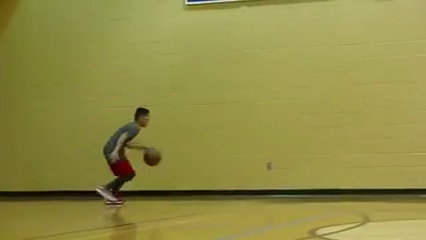
\includegraphics[width=0.25\linewidth]{images/9150.png}} &
    \mcCell{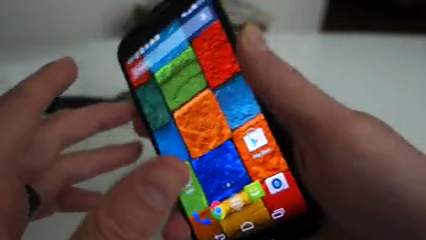
\includegraphics[width=0.25\linewidth]{images/9799.png}} &
    \mcCell{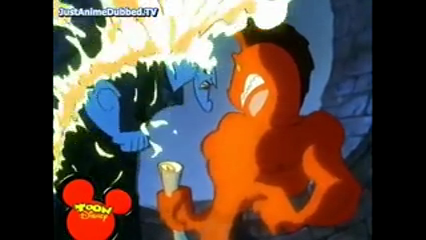
\includegraphics[width=0.25\linewidth]{images/7997.png}} \\
    \textbf{\scriptsize\em M6:} \scriptsize a man is running in a gym &
    \textbf{\scriptsize\em M6:} \scriptsize a person is playing with a rubix cube &
    \textbf{\scriptsize\em M6:} \scriptsize cartoon characters are interacting\\
    \textbf{\scriptsize\em M2:} \scriptsize a man is running&
    \textbf{\scriptsize\em M2:} \scriptsize a man is holding a phone&
    \textbf{\scriptsize\em M2:} \scriptsize a person is playing a video game\\
    \textbf{\scriptsize\em M5:} \scriptsize a man is playing basketball&
    \textbf{\scriptsize\em M5:} \scriptsize a person is playing with a rubix cube &
    \textbf{\scriptsize\em M5:} \scriptsize a group of people are talking\\
  \end{tabular}
  \end{adjustbox}
  \end{center}
  \vspace{-5mm}
  \caption{Sample captions generated for some test set videos by our
          models.}
  \label{fig:capSamps}
\end{figure*}

\begin{table*}[thp]
  \centering
  \begin{adjustbox}{center}
  \newcommand{\bs}{\small\bf}
  \begin{tabular}{||c|c|c|c|c|c|c|c|c|}
    \hline\hline
    \bf\# &\bf init &\bf persist &\bf depth &\bf perplex &\bs BLEU-4 &\bs METEOR &\bs CIDEr &\bs ROUGE-L \\\hline\hline
    M1 & dt  & gCNN+20Categ & 1  & 27.31 & 0.396 & 0.268 & 0.438 & 0.588 \\
    M2 & dt  & gCNN+20Categ & 2  & 27.73 & 0.409 & 0.268 & 0.433 & 0.598 \\
    M3 & dt  & gCNN+20Categ & 3  & 28.44 & 0.370 & 0.262 & 0.397 & 0.575 \\\hline
    M4 & idt & gCNN+20Categ & 2  & 28.13 & 0.398 & 0.268 & 0.432 & 0.587 \\
    M5 & dt  & c3dfc7       & 2  & 29.58 & 0.369 & 0.268 & 0.413 & 0.577 \\\hline
    M6 & \multicolumn{4}{c|}{\em CNN ensemble of best 4 models}
                                  & \bf0.411 & \bf0.277 & \bf0.464 & \bf0.596 \\\hline
    \hline
  \end{tabular}
  \end{adjustbox}
  \label{tab:resVttFeat}
  \caption{Performance of various features and 
    network depths on the validation set of MSR-VTT}
\end{table*}

%% ---------------------------------------------------------------------------

\subsubsection{Challenge Results}

Since the CNN evaluator model performed the best on the validation set, we
submitted that result in the MSR-VTT Challenge.
%%
Our submission appears on the leaderboard as \emph{Aalto}.
%%
The submissions were evaluated on the blind test set using the above mentioned
four automatic metrics.
%%
These results are shown in Table~\ref{tab:resultsTestMet}.
%%
Our submission achieved the best scores in the CIDEr metric and was ranked
overall second considering the average ranking across the metrics.

The submissions were also subject to human evaluation as the automatic metrics
are known to deviate from human judgements.
%%
This was seen in previous captioning challenges in the case of both
image~\cite{CocoChallengeSlides} and
video~\cite{DBLP:journals/corr/RohrbachTRTPLCS16} data.
%%
The human evaluation was based on three criteria: Coherence (C1), Relevance (C2)
and Helpfulness for the blind (C3).
%%
Table~\ref{tab:resultsTestMet} presents the results of the evaluation.
%%
The overall ranking was obtained again by considering the mean ranking across
the three metrics.
%%
As per human judgement, our submission was ranked the first among the 22 entries
in the challenge.

Analyzing the two leaderboards, the automatic metric based one and the human
evaluation based one, we see that the disagreement between the two is relatively
minor, with most teams in the top 10 changing their ranking by only one
position.
%%
This can most likely be attributed to having a large number of 20 reference
captions per video for the evaluation.

\begin{table}[th]
  \centering
  \newcommand{\bs}{\small\bf}
  \scalebox{0.9}{
  \begin{tabular}{||c|c|c|c|c|}
    \hline\hline
    \bf Team  &\bs BLEU-4 &\bs METEOR &\bs CIDEr &\bs ROUGE-L \\\hline\hline
    v2t\_navigator &\bf0.408 &\bf0.282 & 0.448 &\bf0.609 \\
    \bf Aalto      & 0.398 & 0.269 &0.457 & 0.598 \\
    VideoLAB       & 0.391 & 0.277 & 0.441 & 0.606 \\
    ruc-uva        & 0.387 & 0.269 &\bf0.459 & 0.587 \\
    Fudan-ILC      & 0.387 & 0.268 & 0.419 & 0.595 \\\hline
    \hline
  \end{tabular}}
  \label{tab:resultsTestMet}
  \caption{Top 5 teams as per automatic evaluation metrics on the test set}
\end{table}

\begin{table}[th]
  \centering
  \newcommand{\bs}{\small\bf}
  \begin{tabular}{||c|c|c|c|}
    \hline\hline
    \bf Team  &\bs C1 &\bs C2 &\bs C3 \\\hline\hline
    \bf Aalto      & \bf3.263 & 3.104 & \bf3.244\\
    v2t\_navigator & 3.261 & 3.091 & 3.154 \\
    VideoLAB       & 3.237 & \bf3.109 & 3.143 \\
    Fudan-ILC      & 3.185 & 2.999 & 2.979 \\
    ruc-uva        & 3.225 & 2.997 & 2.933 \\\hline
    \hline
  \end{tabular}
  \label{tab:resultsTestHum}
  \caption{Top 5 teams as per human evaluation}
\end{table}

%% ===========================================================================

\section{Conclusions}


\section{Summary of Results}
\fixme{About 2 pages, Fresh writing }
Summarizing results of both image and video, how they are similar and different
(for eg. kinds of mistakes made in video vs image).
